\subsection{Minority allocation, softening, and tied maxima}
Table~\ref{tab:primary} compares all five target representations at the same retained count. Original-four-condition risk--coverage curves and selected/fixed-epoch contrast intervals are retained in the supplement; the direct primary difference curve appears below.
\begin{table}[t]
\caption{Selected-checkpoint risk at 80\% coverage (2,620 of 3,275 images). Risk is mean $\pm$ sample SD; components are mean percentage points}\label{tab:primary}
\centering\begin{tabular}{lrrrr}\toprule
Targets & Risk (\%) & Unsupported & Ambiguity & Excess\\\midrule
Hard & $26.30 \pm 1.04$ & 6.65 & 16.14 & 3.51\\
Tie-hard & $25.82 \pm 0.58$ & 6.67 & 16.03 & 3.13\\
Uniform & $24.06 \pm 0.10$ & 6.41 & 15.41 & 2.24\\
Tie-Uniform & $24.27 \pm 0.17$ & 6.47 & 15.46 & 2.35\\
Soft & $23.68 \pm 0.07$ & 6.55 & 15.01 & 2.13\\
\bottomrule\end{tabular}
Accepted identities differ; components provide accounting, not causal attribution.
\end{table}

The primary Soft-minus-Uniform difference is -0.38 pp (conditional 95\% interval [-0.64, -0.07]). Paired differences for seeds 17, 42, and 89 are -0.35, -0.43, -0.35 pp. Full soft targets yielded lower selective disagreement than the dominant-confidence-preserving uniform-minority control under this matched protocol. The retained original Soft-minus-Hard contrast is -2.61 pp (conditional 95\% interval [-2.98, -2.19]). Tie-hard minus Hard is -0.47 pp (conditional 95\% interval [-0.80, -0.12]); Soft minus Tie-hard is -2.14 pp (conditional 95\% interval [-2.49, -1.76]). These latter intervals are descriptive sensitivities, not additional primary hypothesis tests.


\subsection{Selection sensitivity and label references}
\begin{table}[t]
\caption{Selected versus fixed epoch-12 complete-vote risk at 80\% coverage (\%); means across three paired seeds}\label{tab:sensitivity}
\centering\begin{tabular}{lrr}\toprule
Targets & Selected & Epoch 12\\\midrule
Hard & 26.295 & 24.983\\
Tie-hard & 25.824 & 24.576\\
Uniform & 24.062 & 23.949\\
Tie-Uniform & 24.272 & 23.939\\
Soft & 23.684 & 23.632\\
\bottomrule\end{tabular}

\end{table}

At fixed epoch 12, Soft minus Uniform is -0.32 pp (conditional 95\% interval [-0.63, -0.05]), and Soft minus Hard is -1.35 pp (conditional 95\% interval [-1.72, -1.05]). Table~\ref{tab:sensitivity} keeps both evaluation states visible. This test changes the stopping decision, not the budget or training objective. Reference-specific classification outcomes are separated by both image population and label reference below.

\subsection{Supported mass and the meaning of confidence}
Figure~\ref{fig:mass} separates unsupported mass from ambiguity and excess on each accepted set. Its second panel changes the selection population explicitly rather than silently dropping unsupported votes.
\begin{figure}[t]
\centering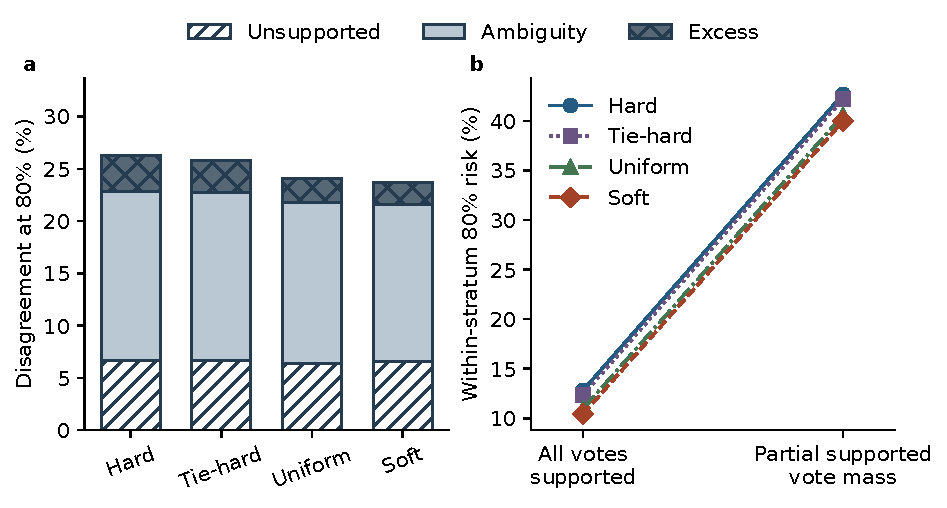
\includegraphics[width=\linewidth]{backbone_followup/figures/Fig3.pdf}
\caption{Original four conditions: (a) three-way mean risk accounting on global 80\% accepted sets. (b) Independent 80\% selection within full- and partial-supported-mass strata; these populations and vertical scales differ from panel (a). Zero-supported-mass images necessarily have complete-vote risk one and are reported in Table~\ref{tab:retention} and Online Resource 1. Neither panel evaluates an expanded-vocabulary model}\label{fig:mass}
\end{figure}
The primary population contains 1,732 fully supported, 1,527 partially supported, and 16 zero-supported-mass images. Within the fully supported stratum, 80\% risk is 10.42\% for Soft and 10.94\% for Uniform. Within the partially supported stratum, 80\% risk is 40.00\% for Soft and 40.58\% for Uniform. These descriptive comparisons address whether the primary contrast is confined to images with unsupported votes; they do not establish why a model assigned a particular score.

\subsection{Fixed-image comparisons and reference effects}
Table~\ref{tab:cross} holds the accepted image set fixed within each column.
\begin{table}[t]
\caption{Cross-evaluation at 80\% coverage: mean complete-vote disagreement (\%) across seeds. Rows hold predictions fixed; columns hold accepted images fixed}\label{tab:cross}
\centering\begin{tabular}{llrr}\toprule
State & Predictor & Uniform set & Soft set\\\midrule
selected & Uniform & 24.062 & 24.037\\
selected & Soft & 24.148 & 23.684\\
epoch12 & Uniform & 23.949 & 23.846\\
epoch12 & Soft & 24.037 & 23.632\\
\bottomrule\end{tabular}

\end{table}

On Uniform-selected images, Soft minus Uniform is +0.085 pp; on Soft-selected images it is -0.352 pp. Within a column, annotations and the floor are identical, so the risk difference is also a category-choice excess difference on that image set. Holding the Uniform predictor fixed, changing from its own set to the Soft set changes risk by -0.025 pp; for the Soft predictor the corresponding change is -0.463 pp. Thus, the own-set contrast is not a consistent category-choice improvement on a fixed image set. Predictor and selector interact; these cross-evaluations are not a unique causal decomposition. The mean Jaccard overlap is 0.8408; individual intersections and overlap fractions are released.
\begin{table}[t]
\caption{Selected-model weighted F1 with population and reference separated; means across three seeds}\label{tab:samef1}
\centering\begin{tabular}{lrrr}\toprule
Targets & Original/all & Original/subset & Crowd/subset\\\midrule
Hard & 0.5658 & 0.6580 & 0.8965\\
Tie-hard & 0.5599 & 0.6572 & 0.9032\\
Uniform & 0.5683 & 0.6642 & 0.9205\\
Tie-Uniform & 0.5662 & 0.6619 & 0.9195\\
Soft & 0.5722 & 0.6685 & 0.9270\\
\bottomrule\end{tabular}
All: 3,275 images; subset: the same 2,484 supported-majority images in the last two columns. No retraining or relabeling is performed.
\end{table}

In Table~\ref{tab:samef1}, the last two columns hold the image population fixed while changing the categorical reference. The first two hold the original-label reference fixed while changing the population. Their differences therefore disentangle two sources of the superficially large original-versus-crowd F1 contrast. The reference confusion matrix is supplied in the supplement; neither reference is treated as emotional truth.
\begin{figure}[t]\centering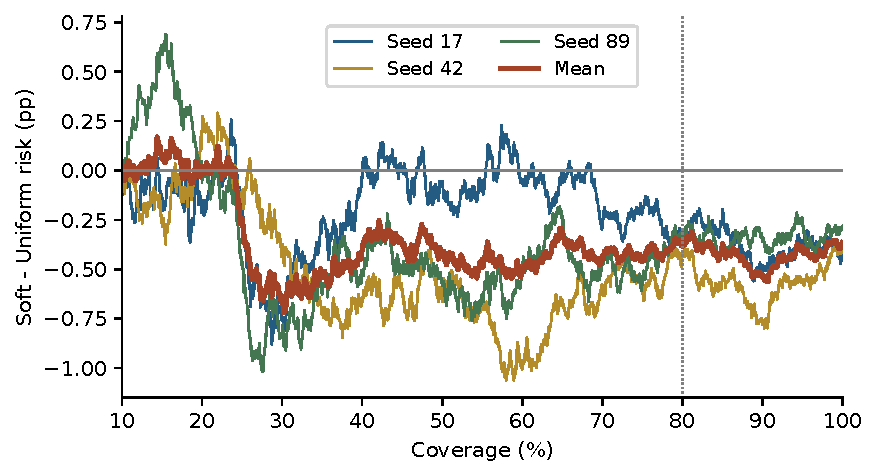
\includegraphics[width=\linewidth]{backbone_followup/figures/RiskDifference.pdf}
\caption{Soft-minus-Uniform complete-vote disagreement versus common coverage. Thin curves are paired seeds; the thick curve is their mean. Curves use each model's own ranking, not identical image sets. The vertical marker identifies the primary 80\% endpoint; this descriptive curve has no simultaneous uncertainty band}\label{fig:difference}\end{figure}
\subsection{Tie-preserving dominant-confidence control}
The tie-preserving comparison is evaluated at both checkpoint states; the later cross-backbone table also reports its contrast intervals.

Selected: paired Soft-minus-Tie-Uniform differences are -0.378, -0.584, -0.802 pp for seeds 17, 42, and 89. The conditional interval lies below zero. Epoch12: paired Soft-minus-Tie-Uniform differences are -0.435, -0.221, -0.263 pp for seeds 17, 42, and 89. The conditional interval lies below zero. This secondary comparison removes canonical tie asymmetry from Uniform but still changes target entropy and class marginals relative to Soft. It cannot isolate a unique minority-category identity mechanism.

Selected epochs and complete training-loss/selection-distance trajectories are supplied in the supplement and ledger. Loss scales differ by target construction and are not directly comparable evidence of better fitting.
\subsection{Retention of unsupported categories}
Table~\ref{tab:retention} retains individual seed counts rather than only a mean ordering.
\begin{table}[t]
\caption{Accepted image counts at global 80\% coverage, seeds 17, 42, 89 in that order. Population sizes: full 1,732; partial 1,527; zero 16}\label{tab:retention}
\centering\begin{tabular}{lrrr}\toprule
Targets & Full mass & Partial mass & Zero mass\\\midrule
Hard & 1499, 1501, 1492 & 1115, 1112, 1122 & 6, 7, 6\\
Tie-hard & 1519, 1494, 1508 & 1092, 1119, 1106 & 9, 7, 6\\
Uniform & 1515, 1527, 1527 & 1098, 1087, 1085 & 7, 6, 8\\
Tie-Uniform & 1529, 1522, 1520 & 1084, 1090, 1095 & 7, 8, 5\\
Soft & 1527, 1527, 1533 & 1081, 1083, 1076 & 12, 10, 11\\
\bottomrule\end{tabular}
Each seed retains 2,620 images in total. Zero-mass images have disagreement one under every supported prediction.
\end{table}

Soft retains 11.00 of the 16 zero-supported-mass images on average, versus 7.00 for Uniform and 6.67 for Tie-Uniform. Better aggregate risk therefore does not imply better rejection of wholly unsupported annotations. These small counts are descriptive, not an estimated deployment failure rate. Contempt, unknown and not-a-face vote-mass breakdowns are supplied separately rather than interpreted as one semantic category.
Before confidence selection, calibration vote mass is 1.797\% contempt, 3.666\% unknown, and 0.262\% not-a-face. Before confidence selection, test vote mass is 1.554\% contempt, 5.667\% unknown, and 0.656\% not-a-face. These are vote fractions, not counts of images; the accepted-set breakdown in the supplement conditions on each ranking.

\subsection{Calibration transfer and finite-sample diagnostics}
\begin{table}[t]
\caption{Calibration-fitted policies applied unchanged to primary testing. Entries are mean coverage / risk (\%); coverage includes empty seeds, risk averages nonempty seeds}\label{tab:policies}
\centering\begin{tabular}{llcc}\toprule
Target & Targets & Empirical & Fixed-grid bound\\\midrule
10\% & Hard & 38.35 / 11.45 (3/3) & 0.00 / -- (0/3)\\
10\% & Tie-hard & 39.17 / 11.93 (3/3) & 0.00 / -- (0/3)\\
10\% & Uniform & 45.99 / 12.22 (3/3) & 0.00 / -- (0/3)\\
10\% & Soft & 49.54 / 13.01 (3/3) & 0.00 / -- (0/3)\\
\addlinespace
20\% & Hard & 68.58 / 22.28 (3/3) & 47.03 / 14.55 (3/3)\\
20\% & Tie-hard & 71.04 / 22.80 (3/3) & 48.05 / 14.61 (3/3)\\
20\% & Uniform & 76.20 / 22.80 (3/3) & 57.49 / 16.11 (3/3)\\
20\% & Soft & 76.88 / 22.56 (3/3) & 60.39 / 16.60 (3/3)\\
\addlinespace
30\% & Hard & 98.06 / 32.39 (3/3) & 82.01 / 26.92 (3/3)\\
30\% & Tie-hard & 99.47 / 32.37 (3/3) & 85.41 / 27.54 (3/3)\\
30\% & Uniform & 99.94 / 31.46 (3/3) & 88.41 / 27.11 (3/3)\\
30\% & Soft & 99.91 / 31.07 (3/3) & 89.57 / 27.01 (3/3)\\
\bottomrule\end{tabular}
\smallskip\par\footnotesize Parentheses give nonempty test seeds. An empty policy has undefined risk. Neither a nominal target nor the bound's unverified independence/unchanged-population assumptions establish a deployment guarantee. Different achieved risks are not an equal-risk coverage comparison.
\end{table}

Table~\ref{tab:policies} includes every target and empty-policy outcome. Figure~\ref{fig:transfer} partitions the empirical policy's accepted-population risk change.
\begin{figure}[t]
\centering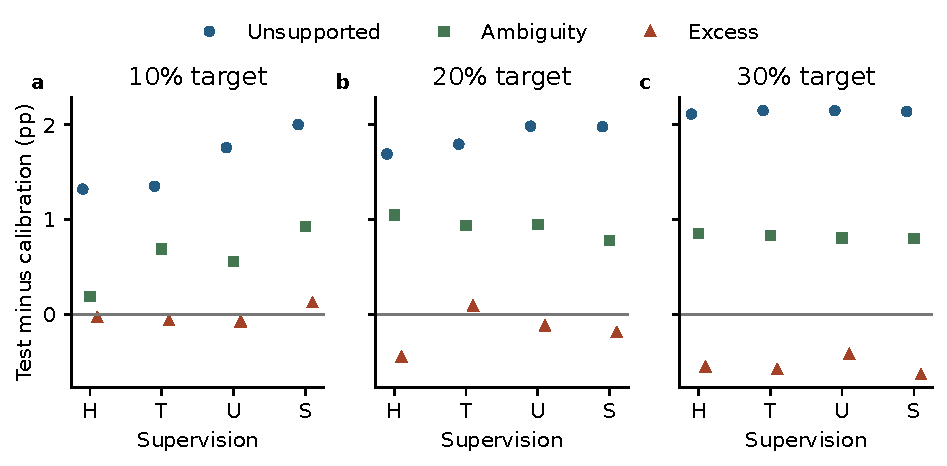
\includegraphics[width=\linewidth]{backbone_followup/figures/Fig4.pdf}
\caption{Mean test-minus-calibration differences in unsupported mass, supported ambiguity, and excess error for empirical thresholds. Their sum is the risk gap, not a causal attribution. H: Hard; T: Tie-hard; U: Uniform; S: Soft. The three target panels share a vertical scale. Means use paired nonempty calibration/test selections}\label{fig:transfer}
\end{figure}
Across the original four conditions, 36 of 36 nonempty empirical test operating points exceed their nominal targets. These overlapping outcomes are not independent Bernoulli trials. At the 10\% target, Hard has 38.35\% mean coverage and 11.45\% mean achieved risk. At the 10\% target, Soft has 49.54\% mean coverage and 13.01\% mean achieved risk. Different achieved risks prevent interpreting this as greater coverage at equal risk.

Before confidence selection, the annotation floor is 23.70\% in calibration and 26.67\% in testing: a +2.97 pp difference. Unsupported mass changes from 5.72\% to 7.88\%; the remaining floor difference is supported-category ambiguity. Thus, these populations differ in annotation composition even before a model supplies a ranking.

For Soft at the nominal 20\% target, the accepted test-minus-calibration risk gap is +2.57 pp, comprising +1.98 pp unsupported mass, +0.78 pp supported ambiguity, and -0.19 pp excess. The figure and ledger supply the analogous accounting for every condition and target; this arithmetic does not identify independent causal contributions.

For Hard, the 20\% calibration-half-split holdout-minus-fit risk gap averages +0.05 pp over 300 nonempty seed--split outcomes (descriptive 5th--95th percentiles -2.33 to +2.59 pp). For Tie-hard, the 20\% calibration-half-split holdout-minus-fit risk gap averages +0.18 pp over 300 nonempty seed--split outcomes (descriptive 5th--95th percentiles -2.34 to +2.77 pp). For Uniform, the 20\% calibration-half-split holdout-minus-fit risk gap averages +0.19 pp over 300 nonempty seed--split outcomes (descriptive 5th--95th percentiles -2.02 to +2.62 pp). For Soft, the 20\% calibration-half-split holdout-minus-fit risk gap averages +0.17 pp over 300 nonempty seed--split outcomes (descriptive 5th--95th percentiles -2.00 to +2.43 pp). The complete target-specific resamples are released. These diagnostics reveal within-calibration variability and accepted-population differences, but cannot uniquely separate distribution shift, finite-sample fluctuation, and threshold-search effects.
The fixed-grid comparator yields 24 nonempty test operating points, of which 0 exceed their nominal targets. It abstains completely at the 10\% target for every condition and seed. Its observed conservatism therefore has a concrete coverage cost; these outcomes do not verify its population assumptions.

\subsection{Robustness across two backbone families}
The nine new ResNet runs keep the supervision contrast matched within each seed. Table~\ref{tab:backbones} reports both selected and epoch-12 contrasts; absolute ResNet risks are in the supplement.
\begin{table}[t]
\caption{Within-backbone Soft-minus-control disagreement at 80\% coverage (percentage points). Intervals condition on fitted models, three seeds, observed pixels and votes}\label{tab:backbones}
\centering\begin{tabular}{lllrr}\toprule
Backbone & State & Control & Difference & 95\% interval\\\midrule
Swin-T & selected & Uniform & -0.378 & [-0.644, -0.073]\\
Swin-T & selected & Tie-Uniform & -0.588 & [-0.830, -0.281]\\
Swin-T & epoch12 & Uniform & -0.317 & [-0.626, -0.050]\\
Swin-T & epoch12 & Tie-Uniform & -0.307 & [-0.585, -0.024]\\
ResNet-18 & selected & Uniform & +0.173 & [-0.167, +0.455]\\
ResNet-18 & selected & Tie-Uniform & +0.042 & [-0.258, +0.343]\\
ResNet-18 & epoch12 & Uniform & +0.170 & [-0.157, +0.467]\\
ResNet-18 & epoch12 & Tie-Uniform & +0.190 & [-0.126, +0.515]\\
\bottomrule\end{tabular}\par
\smallskip
ResNet comparisons are adaptive secondary robustness checks, not independent-image confirmation or architecture comparisons.\par
\end{table}

Selected ResNet Soft-minus-Uniform differences for seeds 17, 42 and 89 are +0.347, +0.137, +0.034 pp. Selected ResNet Soft-minus-Tie-Uniform differences for seeds 17, 42 and 89 are +0.118, +0.115, -0.107 pp. Epoch-12 ResNet Soft-minus-Uniform differences for seeds 17, 42 and 89 are +0.073, +0.489, -0.050 pp. Epoch-12 ResNet Soft-minus-Tie-Uniform differences for seeds 17, 42 and 89 are +0.324, +0.118, +0.126 pp. 
On Uniform-selected images the ResNet fixed-set difference is +0.445 pp; on Soft-selected images it is -0.412 pp. On Tie-Uniform-selected images the ResNet fixed-set difference is +0.613 pp; on Soft-selected images it is -0.024 pp. The full fixed-set matrices, overlaps, reference F1, retention and learning trajectories are provided in the supplement and ledger. These comparisons extend architecture sensitivity but retain the same images, annotations and adaptive research history.
\begin{figure}[t]\centering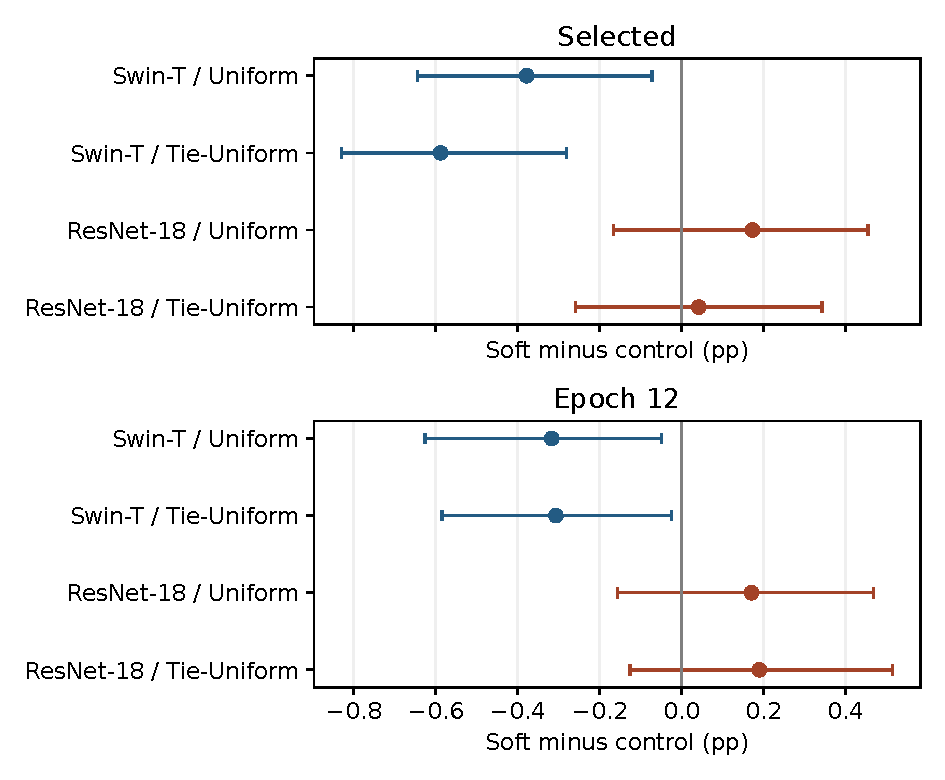
\includegraphics[width=\linewidth]{backbone_followup/figures/BackboneContrasts.pdf}
\caption{Soft-minus-control risk at 80\% own-ranking coverage in two backbone families. Conditional pixel-cluster intervals do not represent seed-population uncertainty or external-domain confirmation. Negative values favor Soft; the figure does not rank architectures}\label{fig:backbones}\end{figure}
